\documentclass[12pt,a4paper]{extarticle}
\usepackage[utf8]{inputenc}
\usepackage[T5]{fontenc}
\usepackage{geometry}
\geometry{a4paper, left=1.5cm, right=1cm, top=1.5cm, bottom=1.5cm, headheight=20pt, headsep=15pt, footskip=28pt}
\usepackage{enumitem}
\usepackage{amsmath}
\usepackage{amssymb}
\usepackage{diagbox}
\usepackage{colortbl} % Sửa lỗi \arrayrulecolor
\usepackage{array}    % Hỗ trợ định dạng cột m{2cm}
\usepackage[most]{tcolorbox}
\newcommand{\khongxacdinh}{\text{KXĐ}}
\newcommand{\blackbox}[1]{\texorpdfstring{\fcolorbox{black}{black}{\textcolor{white}{#1}}}{#1}}
\usepackage{tikz}
\definecolor{bookblue}{RGB}{58,90,172}
\definecolor{book}{RGB}{58,90,172}
\definecolor{myblue}{RGB}{200,40,40}
\newcommand{\bluecheck}{\textcolor{myblue}{\checkmark}}
\newtcolorbox{formulaBox}{colback=gray!5,colframe=bookblue,boxrule=0.8pt,arc=2mm}
\newtcolorbox{notebox}{colback=blue!3,colframe=myblue,boxrule=0.8pt,arc=2mm}
\usetikzlibrary{patterns, patterns.meta} % Thêm patterns.meta vào đây
% Gọi package nằm trong thư mục con template
\usepackage{../template/mngocbox}

\begin{document}

% Sử dụng ngoặc vuông [...] để thay đổi linh hoạt các thông số
\makeheadbox[headerright={Chương 1},chude={Bài 4},tieude={Các đồ thị hàm số kinh điển},dinhdang={Giải tích},lop={12 },gv={Nguyễn Lê Minh Ngọc}]
\vspace{2em}
\makeheading{I}{Kiến thức cần nhớ}
\section*{I. Đồ thị hàm số bậc ba $y = ax^3 + bx^2 + cx + d$}
Cho hàm số $f(x) = ax^3 + bx^2 + cx + d$ ($a \neq 0$). 
Đạo hàm: $f'(x) = 3ax^2 + 2bx + c$ có biệt thức $\Delta' = b^2 - 3ac$.
\subsection*{1. Các dạng đồ thị dựa trên hệ số $a$ và $\Delta'$}
\noindent\textbf{Trường hợp $a > 0$:}
\begin{center}
    \begin{minipage}{0.32\textwidth}
        \centering
        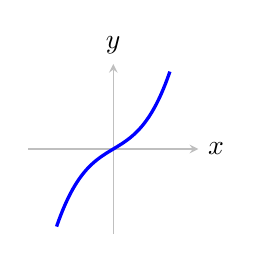
\begin{tikzpicture}[scale=0.9, >=stealth]
            \draw[->, gray!50] (-1.2,0) -- (1.2,0) node[right, black] {$x$};
            \draw[->, gray!50] (0,-1.2) -- (0,1.2) node[above, black] {$y$};
            \draw[blue, very thick, domain=-0.8:0.8, samples=50] plot (\x, {1.2*(\x^3 + 0.5*\x)});
        \end{tikzpicture}
        \par\vspace{0.2cm}
        $\Delta' < 0$
    \end{minipage}
    \hfill
    \begin{minipage}{0.32\textwidth}
        \centering
        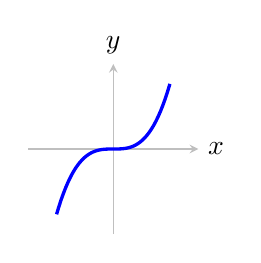
\begin{tikzpicture}[scale=0.9, >=stealth]
            \draw[->, gray!50] (-1.2,0) -- (1.2,0) node[right, black] {$x$};
            \draw[->, gray!50] (0,-1.2) -- (0,1.2) node[above, black] {$y$};
            \draw[blue, very thick, domain=-0.8:0.8, samples=50] plot (\x, {1.8*\x^3});
        \end{tikzpicture}
        \par\vspace{0.2cm}
        $\Delta' = 0$
    \end{minipage}
    \hfill
    \begin{minipage}{0.32\textwidth}
        \centering
        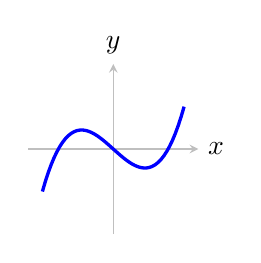
\begin{tikzpicture}[scale=0.9, >=stealth]
            \draw[->, gray!50] (-1.2,0) -- (1.2,0) node[right, black] {$x$};
            \draw[->, gray!50] (0,-1.2) -- (0,1.2) node[above, black] {$y$};
            \draw[blue, very thick, domain=-1.0:1.0, samples=50] plot (\x, {1.5*(\x^3 - 0.6*\x)});
        \end{tikzpicture}
        \par\vspace{0.2cm}
        $\Delta' > 0$
    \end{minipage}
\end{center}
\vspace{1em}
\noindent\textbf{Trường hợp $a < 0$:}
\begin{center}
    \begin{minipage}{0.32\textwidth}
        \centering
        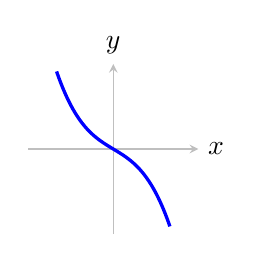
\begin{tikzpicture}[scale=0.9, >=stealth]
            \draw[->, gray!50] (-1.2,0) -- (1.2,0) node[right, black] {$x$};
            \draw[->, gray!50] (0,-1.2) -- (0,1.2) node[above, black] {$y$};
            \draw[blue, very thick, domain=-0.8:0.8, samples=50] plot (\x, {-1.2*(\x^3 + 0.5*\x)});
        \end{tikzpicture}
        \par\vspace{0.2cm}
        $\Delta' < 0$
    \end{minipage}
    \hfill
    \begin{minipage}{0.32\textwidth}
        \centering
        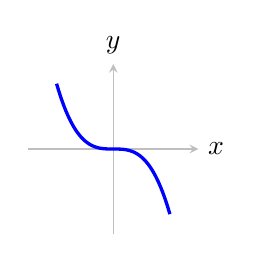
\begin{tikzpicture}[scale=0.9, >=stealth]
            \draw[->, gray!50] (-1.2,0) -- (1.2,0) node[right, black] {$x$};
            \draw[->, gray!50] (0,-1.2) -- (0,1.2) node[above, black] {$y$};
            \draw[blue, very thick, domain=-0.8:0.8, samples=50] plot (\x, {-1.8*\x^3});
        \end{tikzpicture}
        \par\vspace{0.2cm}
        $\Delta' = 0$
    \end{minipage}
    \hfill
    \begin{minipage}{0.32\textwidth}
        \centering
        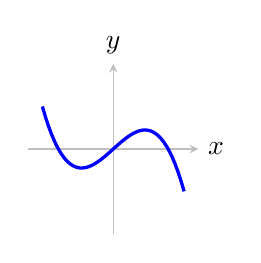
\begin{tikzpicture}[scale=0.9, >=stealth]
            \draw[->, gray!50] (-1.2,0) -- (1.2,0) node[right, black] {$x$};
            \draw[->, gray!50] (0,-1.2) -- (0,1.2) node[above, black] {$y$};
            \draw[blue, very thick, domain=-1.0:1.0, samples=50] plot (\x, {-1.5*(\x^3 - 0.6*\x)});
        \end{tikzpicture}
        \par\vspace{0.2cm}
        $\Delta' > 0$
    \end{minipage}
\end{center}
\subsection*{2. Các tính chất quan trọng}
\begin{itemize}[leftmargin=*]
    \item \textbf{Điểm uốn của đồ thị:} Điểm uốn của đồ thị hàm số bậc ba là tâm đối xứng của đồ thị.
    \begin{itemize}
        \item Xét đạo hàm cấp hai: $f''(x) = 6ax + 2b$.
        \item Giải phương trình $f''(x) = 0 \Leftrightarrow x = \frac{-b}{3a}$.
        \item Điểm $U\left(-\frac{b}{3a}; f\left(-\frac{b}{3a}\right)\right)$ là điểm uốn của đồ thị.
    \end{itemize}
    \item \textbf{Cực trị:} Đồ thị hàm số bậc ba có thể:
    \begin{itemize}
        \item Không có cực trị (khi $\Delta' \le 0$).
        \item Hoặc có đúng 2 điểm cực trị (khi $\Delta' > 0$).
    \end{itemize}
\end{itemize}
\section*{II. Đồ thị hàm số bậc nhất trên bậc nhất}

\subsection*{1. Tóm tắt kiến thức}

Xét hàm số $f(x) = \dfrac{ax + b}{cx + d}$ ($c \neq 0$).

\begin{center}
    % Đồ thị 1: ad - bc < 0
    \begin{minipage}{0.48\textwidth}
        \centering
        \begin{tikzpicture}[scale=1.2, >=stealth]
            % Đường tiệm cận nét đứt
            \draw[dashed, thick] (-2.2, 0) -- (2.2, 0);
            \draw[dashed, thick] (0, -2.2) -- (0, 2.2);
            
            % Nhánh trái dưới (x < 0)
            \draw[blue, very thick, domain=-2.0:-0.2, samples=100] plot (\x, {0.4/\x});
            % Nhánh phải trên (x > 0)
            \draw[blue, very thick, domain=0.2:2.0, samples=100] plot (\x, {0.4/\x});
        \end{tikzpicture}
        \par\vspace{0.3cm}
        \textbf{$ad - bc < 0$}
    \end{minipage}
    \hfill
    % Đồ thị 2: ad - bc > 0
    \begin{minipage}{0.48\textwidth}
        \centering
        \begin{tikzpicture}[scale=1.2, >=stealth]
            % Đường tiệm cận nét đứt
            \draw[dashed, thick] (-2.2, 0) -- (2.2, 0);
            \draw[dashed, thick] (0, -2.2) -- (0, 2.2);
            
            % Nhánh trái trên (x < 0)
            \draw[blue, very thick, domain=-2.0:-0.2, samples=100] plot (\x, {-0.4/\x});
            % Nhánh phải dưới (x > 0)
            \draw[blue, very thick, domain=0.2:2.0, samples=100] plot (\x, {-0.4/\x});
        \end{tikzpicture}
        \par\vspace{0.3cm}
        \textbf{$ad - bc > 0$}
    \end{minipage}
\end{center}

\vspace{1.5em}

\noindent\textbf{$\Rightarrow$ Nhận xét:}
\begin{itemize}[leftmargin=*, label=$\bigstar$, itemsep=0.5em]
    \item \textbf{Đồ thị hàm số có 2 đường tiệm cận:}
    \begin{itemize}[label=$\bullet$, itemsep=0.3em]
        \item Tiệm cận ngang: $y = \dfrac{a}{c}$.
        \item Tiệm cận đứng: $x = -\dfrac{d}{c}$.
    \end{itemize}
    \item \textbf{Tâm đối xứng:} Giao điểm hai đường tiệm cận là tâm đối xứng của đồ thị hàm số, kí hiệu là $I\left(-\dfrac{d}{c}; \dfrac{a}{c}\right)$.
    \item \textbf{Tính đơn điệu:} Hàm số $f(x)$ luôn đồng biến (hoặc nghịch biến) trên từng khoảng xác định.
\end{itemize}
\section*{III. Đồ thị hàm số bậc hai trên bậc nhất}

\subsection*{1. Tóm tắt kiến thức}

Xét hàm số $f(x) = \dfrac{ax^2 + bx + c}{px + q}$ với $a \neq 0, p \neq 0$, đa thức tử không chia hết cho đa thức mẫu.

\vspace{1em}

\noindent\textbf{Các dạng đồ thị tiêu biểu:}
\begin{center}
    % Hàng 1
    \begin{minipage}{0.48\textwidth}
        \centering
        \begin{tikzpicture}[scale=0.9, >=stealth]
            % Tiệm cận đứng và xiên
            \draw[dashed, thick] (0, -2.2) -- (0, 2.2);
            \draw[dashed, thick] (-2.2, -1.1) -- (2.2, 1.1);
            \fill (0,0) circle (1.5pt) node[left=2pt] {$I$};
            
            % Nhánh trái dưới (x < 0)
            \draw[blue, very thick, domain=-2.0:-0.15, samples=100] plot (\x, {0.5*\x + 0.15/\x});
            % Nhánh phải trên (x > 0)
            \draw[blue, very thick, domain=0.15:2.0, samples=100] plot (\x, {0.5*\x + 0.15/\x});
        \end{tikzpicture}
    \end{minipage}
    \hfill
    \begin{minipage}{0.48\textwidth}
        \centering
        \begin{tikzpicture}[scale=0.9, >=stealth]
            % Tiệm cận đứng và xiên
            \draw[dashed, thick] (0, -2.2) -- (0, 2.2);
            \draw[dashed, thick] (-2.2, 1.1) -- (2.2, -1.1);
            \fill (0,0) circle (1.5pt) node[left=2pt] {$I$};
            
            % Nhánh trái trên (x < 0)
            \draw[blue, very thick, domain=-2.0:-0.15, samples=100] plot (\x, {-0.5*\x - 0.15/\x});
            % Nhánh phải dưới (x > 0)
            \draw[blue, very thick, domain=0.15:2.0, samples=100] plot (\x, {-0.5*\x - 0.15/\x});
        \end{tikzpicture}
    \end{minipage}

    \vspace{1.5em}

    % Hàng 2
    \begin{minipage}{0.48\textwidth}
        \centering
        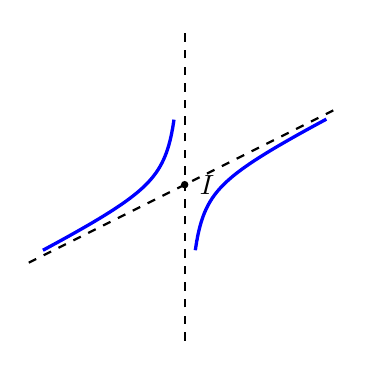
\begin{tikzpicture}[scale=0.9, >=stealth]
            % Tiệm cận đứng và xiên
            \draw[dashed, thick] (0, -2.2) -- (0, 2.2);
            \draw[dashed, thick] (-2.2, -1.1) -- (2.2, 1.1);
            \fill (0,0) circle (1.5pt) node[right=2pt] {$I$};
            
            % Nhánh trái (x < 0)
            \draw[blue, very thick, domain=-2.0:-0.15, samples=100] plot (\x, {0.5*\x - 0.15/\x});
            % Nhánh phải (x > 0)
            \draw[blue, very thick, domain=0.15:2.0, samples=100] plot (\x, {0.5*\x - 0.15/\x});
        \end{tikzpicture}
    \end{minipage}
    \hfill
    \begin{minipage}{0.48\textwidth}
        \centering
        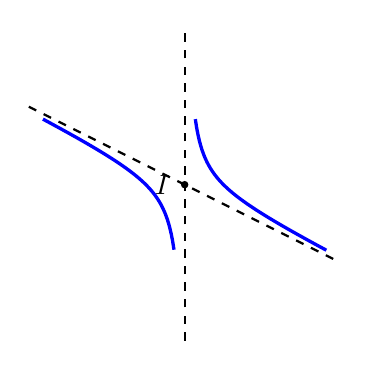
\begin{tikzpicture}[scale=0.9, >=stealth]
            % Tiệm cận đứng và xiên
            \draw[dashed, thick] (0, -2.2) -- (0, 2.2);
            \draw[dashed, thick] (-2.2, 1.1) -- (2.2, -1.1);
            \fill (0,0) circle (1.5pt) node[left=2pt] {$I$};
            
            % Nhánh trái (x < 0)
            \draw[blue, very thick, domain=-2.0:-0.15, samples=100] plot (\x, {-0.5*\x + 0.15/\x});
            % Nhánh phải (x > 0)
            \draw[blue, very thick, domain=0.15:2.0, samples=100] plot (\x, {-0.5*\x + 0.15/\x});
        \end{tikzpicture}
    \end{minipage}
\end{center}

\vspace{1.5em}

\noindent\textbf{$\Rightarrow$ Nhận xét:} Đồ thị hàm số có 2 đường tiệm cận:
\begin{itemize}[leftmargin=*, label=$\bullet$, itemsep=0.5em]
    \item \textbf{Tiệm cận xiên:} Viết lại $f(x) = mx + n + \dfrac{k}{px + q}$ ($m \neq 0$) thì đồ thị hàm số nhận đường thẳng $y = mx + n$ làm đường tiệm cận xiên.
    \item \textbf{Tiệm cận đứng:} $x = -\dfrac{q}{p}$.
    \item Đồ thị hàm số nhận giao điểm của hai đường tiệm cận làm tâm đối xứng.
    \item Đồ thị hàm số nhận đường phân giác của các góc tạo bởi hai đường tiệm cận này làm các trục đối xứng.
\end{itemize}

\vspace{2em}

\noindent\textbf{\Large\color{blue}Lưu ý}

\subsection*{1. Phương trình đường thẳng đi qua hai điểm cực trị}

\begin{doublelinebox}
    Nếu đồ thị hàm số $y = f(x) = \dfrac{ax^2 + bx + c}{px + q}$ có 2 điểm cực trị là $A$ và $B$, thì phương trình đường thẳng $AB$ là:
    \[
    y = \frac{(ax^2 + bx + c)'}{(px + q)'} = \frac{2ax + b}{p}
    \]
\end{doublelinebox}



\subsection*{2. Mẹo kiểm tra nhanh xem hàm số có cực trị hay không}
\begin{doublelinebox}
    Xét hàm số $f(x) = \dfrac{ax^2 + bx + c}{px + q}$ với $a \neq 0, p \neq 0$, đa thức tử không chia hết cho đa thức mẫu.\\
    Đặt $g(x) = ax^2 + bx + c$.
    \begin{itemize}[leftmargin=*, label=\color{blue}$\bullet$, itemsep=0.5em]
        \item Nếu $a \cdot g\left(-\dfrac{q}{p}\right) > 0$ thì hàm số $f(x)$ có 2 điểm cực trị.
        \item Nếu $a \cdot g\left(-\dfrac{q}{p}\right) \le 0$ thì hàm số $f(x)$ không có cực trị.
    \end{itemize}
\end{doublelinebox}
\end{document}